\section{Heap}

\begin{frame}
	\frametitle{Heap}
	A heap is a structure with (mainly) two operations:
	\begin{itemize}
		\item \texttt{push}: Add an element to the heap $O(\log n)$.
		\item \texttt{pop}: remove and return the biggest/greater/... element from the heap $O(\log n)$.
	\end{itemize}
	\pause How to implement it?
	\pause With a tree, of course!
\end{frame}

\begin{frame}
	\frametitle{The heap property}
	Remember the binary search tree property?\\
	\vspace{1cm}
	\textbf{(max) Heap property}: Childrens of a node in a heap tree are $\leq$ than the node itself.\\
	\vspace{1cm}
	One of the most simple and efficient heap implementation are complete binary heap. Two more rules then:
	\begin{itemize}
		\item The tree is a binary one ($\leq$ 2 children per node)
		\item The tree is "complete": all levels of the tree are full of nodes but the last one, on which leaves are on the left
	\end{itemize}
\end{frame}


\begin{frame}
	\frametitle{Which are valid complete binary heap trees?}
	
	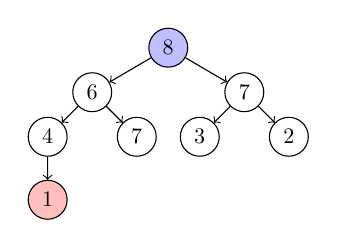
\begin{tikzpicture}[->,nodes={draw, circle,scale=0.8},scale=0.8]
	\node (a8) [fill = blue!25] {8};
	\node (a6) [below left of = a8, xshift=-0.5cm] {6};
	\node (a7) [below right of = a8, xshift=0.5cm]{7};
	\node (a4) [below left of = a6]{4};
	\node (a5) [below right of = a6]{7};
	\node (a3) [below left of = a7]{3};
	\node (a2) [below right of = a7]{2};
	\node (a1) [below of = a4, fill = red!25]{1};
	
	\draw (a8) -> (a7);
	\draw (a8) -> (a6); 
	\draw (a6) -> (a4);
	\draw (a6) -> (a5);
	\draw (a7) -> (a3);
	\draw (a7) -> (a2);
	\draw (a4) -> (a1);
	\end{tikzpicture} \only<2>{(heap property not respected on 6-7)}
	
	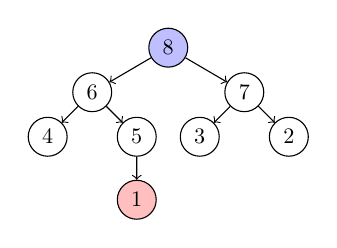
\begin{tikzpicture}[->,nodes={draw, circle,scale=0.8},scale=0.8]
	\node (a8) [fill = blue!25] {8};
	\node (a6) [below left of = a8, xshift=-0.5cm] {6};
	\node (a7) [below right of = a8, xshift=0.5cm]{7};
	\node (a4) [below left of = a6]{4};
	\node (a5) [below right of = a6]{5};
	\node (a3) [below left of = a7]{3};
	\node (a2) [below right of = a7]{2};
	\node (a1) [below of = a5, fill = red!25]{1};
	
	\draw (a8) -> (a7);
	\draw (a8) -> (a6); 
	\draw (a6) -> (a4);
	\draw (a6) -> (a5);
	\draw (a7) -> (a3);
	\draw (a7) -> (a2);
	\draw (a5) -> (a1);
	\end{tikzpicture} \only<2>{(leaf 1 not on left)}
	
	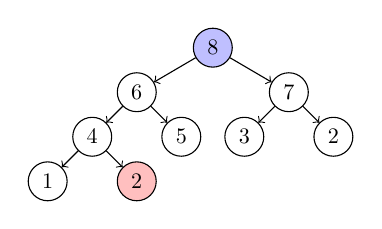
\begin{tikzpicture}[->,nodes={draw, circle,scale=0.8},scale=0.8]
	\node (a8) [fill = blue!25] {8};
	\node (a6) [below left of = a8, xshift=-0.5cm] {6};
	\node (a7) [below right of = a8, xshift=0.5cm]{7};
	\node (a4) [below left of = a6]{4};
	\node (a5) [below right of = a6]{5};
	\node (a3) [below left of = a7]{3};
	\node (a2) [below right of = a7]{2};
	\node (a1) [below left of = a4]{1};
	\node (a22) [below right of = a4, fill = red!25]{2};
	
	\draw (a8) -> (a7);
	\draw (a8) -> (a6); 
	\draw (a6) -> (a4);
	\draw (a6) -> (a5);
	\draw (a7) -> (a3);
	\draw (a7) -> (a2);
	\draw (a4) -> (a1);
	\draw (a4) -> (a22);
	\end{tikzpicture} \only<2>{(valid!)}
\end{frame}

\begin{frame}
	\frametitle{Storing a complete tree}
	Storing a complete tree is easy: use an array (or a vector)!
	\vspace{0.5cm}
	\begin{center}
		\begin{tabular}{ccccccccc}
			0 & 1 & 2 & 3 & 4 & 5 & 6 & 7 & 8\\
		\end{tabular}
		\begin{tabular}{|c|c|c|c|c|c|c|c|c|}
			\hline
			a & b & c & d & e & f & g & h & i\\
			\hline
		\end{tabular}
		
		\vspace{0.5cm}
		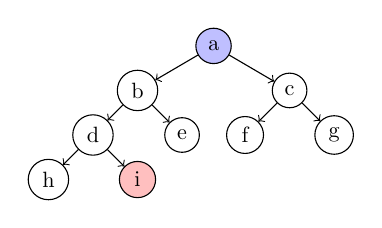
\begin{tikzpicture}[->,nodes={draw, circle,scale=0.8},scale=0.8]
		\node (a8) [fill = blue!25] {a};
		\node (a6) [below left of = a8, xshift=-0.5cm] {b};
		\node (a7) [below right of = a8, xshift=0.5cm]{c};
		\node (a4) [below left of = a6]{d};
		\node (a5) [below right of = a6]{e};
		\node (a3) [below left of = a7]{f};
		\node (a2) [below right of = a7]{g};
		\node (a1) [below left of = a4]{h};
		\node (a22) [below right of = a4, fill = red!25]{i};
		
		\draw (a8) -> (a7);
		\draw (a8) -> (a6); 
		\draw (a6) -> (a4);
		\draw (a6) -> (a5);
		\draw (a7) -> (a3);
		\draw (a7) -> (a2);
		\draw (a4) -> (a1);
		\draw (a4) -> (a22);
		\end{tikzpicture}
	\end{center}
	If $p$ is the idx of the parent in the array, idx of the children are:
	\begin{itemize}
		\item $2p+1$
		\item $2p+2$
	\end{itemize}
	Next node to be created is always at the end of the array!
\end{frame}

\begin{frame}
	\frametitle{Adding a new element}
	\begin{enumerate}
		\item Add new element at the end of the tree
		\item If parent does not respect the heap property (== is lesser than the new node)
		\begin{enumerate}
			\item Exchange the node and its parent
			\item Repeat from 2.
		\end{enumerate}
	\end{enumerate}
\end{frame}

\begin{frame}
	\frametitle{Adding a new element}
	Adding $7$:
	\begin{center}
	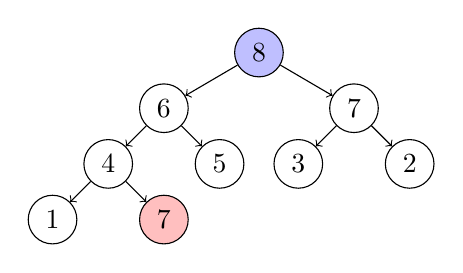
\begin{tikzpicture}[->,nodes={draw, circle}]
	\node (a8) [fill = blue!25] {8};
	\node (a6) [below left of = a8, xshift=-0.5cm] {6};
	\node (a7) [below right of = a8, xshift=0.5cm]{7};
	\node (a4) [below left of = a6]{4};
	\node (a5) [below right of = a6]{5};
	\node (a3) [below left of = a7]{3};
	\node (a2) [below right of = a7]{2};
	\node (a1) [below left of = a4]{1};
	\node (n7) [below right of = a4, fill = red!25]{7};
	\draw (a8) -> (a7);
	\draw (a8) -> (a6); 
	\draw (a6) -> (a4);
	\draw (a6) -> (a5);
	\draw (a7) -> (a3);
	\draw (a7) -> (a2);
	\draw (a4) -> (a1);
	\draw (a4) -> (n7);
	\end{tikzpicture}
	\end{center}
\end{frame}

\begin{frame}
	\frametitle{Adding a new element}
	Adding $7$:
	\begin{center}
		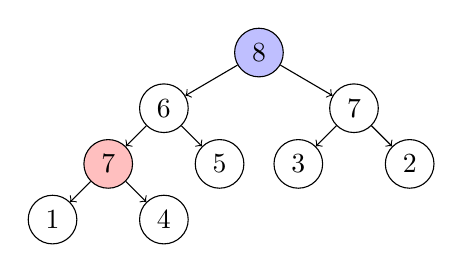
\begin{tikzpicture}[->,nodes={draw, circle}]
		\node (a8) [fill = blue!25] {8};
		\node (a6) [below left of = a8, xshift=-0.5cm] {6};
		\node (a7) [below right of = a8, xshift=0.5cm]{7};
		\node (a4) [below left of = a6, fill = red!25]{7};
		\node (a5) [below right of = a6]{5};
		\node (a3) [below left of = a7]{3};
		\node (a2) [below right of = a7]{2};
		\node (a1) [below left of = a4]{1};
		\node (n7) [below right of = a4]{4};
		\draw (a8) -> (a7);
		\draw (a8) -> (a6); 
		\draw (a6) -> (a4);
		\draw (a6) -> (a5);
		\draw (a7) -> (a3);
		\draw (a7) -> (a2);
		\draw (a4) -> (a1);
		\draw (a4) -> (n7);
		\end{tikzpicture}
	\end{center}
\end{frame}

\begin{frame}
	\frametitle{Adding a new element}
	Adding $7$:
	\begin{center}
		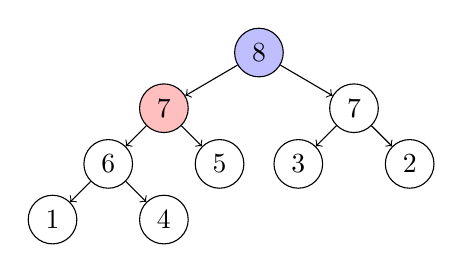
\begin{tikzpicture}[->,nodes={draw, circle}]
		\node (a8) [fill = blue!25] {8};
		\node (a6) [below left of = a8, xshift=-0.5cm, fill = red!25] {7};
		\node (a7) [below right of = a8, xshift=0.5cm]{7};
		\node (a4) [below left of = a6]{6};
		\node (a5) [below right of = a6]{5};
		\node (a3) [below left of = a7]{3};
		\node (a2) [below right of = a7]{2};
		\node (a1) [below left of = a4]{1};
		\node (n7) [below right of = a4]{4};
		\draw (a8) -> (a7);
		\draw (a8) -> (a6); 
		\draw (a6) -> (a4);
		\draw (a6) -> (a5);
		\draw (a7) -> (a3);
		\draw (a7) -> (a2);
		\draw (a4) -> (a1);
		\draw (a4) -> (n7);
		\end{tikzpicture}
	\end{center}
\end{frame}

\begin{frame}
	\frametitle{Adding a new element}
	Adding $7$:
	\begin{center}
		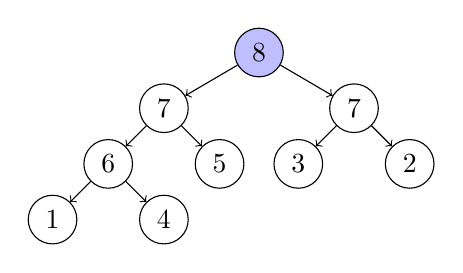
\begin{tikzpicture}[->,nodes={draw, circle}]
		\node (a8) [fill = blue!25] {8};
		\node (a6) [below left of = a8, xshift=-0.5cm] {7};
		\node (a7) [below right of = a8, xshift=0.5cm]{7};
		\node (a4) [below left of = a6]{6};
		\node (a5) [below right of = a6]{5};
		\node (a3) [below left of = a7]{3};
		\node (a2) [below right of = a7]{2};
		\node (a1) [below left of = a4]{1};
		\node (n7) [below right of = a4]{4};
		\draw (a8) -> (a7);
		\draw (a8) -> (a6); 
		\draw (a6) -> (a4);
		\draw (a6) -> (a5);
		\draw (a7) -> (a3);
		\draw (a7) -> (a2);
		\draw (a4) -> (a1);
		\draw (a4) -> (n7);
		\end{tikzpicture}
	\end{center}
\end{frame}

\begin{frame}
	\frametitle{Removing the first element}
	\begin{enumerate}
		\item Save somewhere the root of the tree to return it later
		\item Take the last node value, and put it at the top of the tree
		\item Three cases then:
			\begin{itemize}
				\item If the heap property is respected (node $\geq$ its children), return
				\item If one of the children is $>$ the node, swap them and repeat from 3.
				\item If both children are $>$ the node, swap with the greatest child and repeat from 3.
			\end{itemize}
	\end{enumerate}
\end{frame}

\begin{frame}
	\frametitle{Removing the first element}
	Step 1: store the root somewhere (remember: root was 8)
	
	\begin{center}
		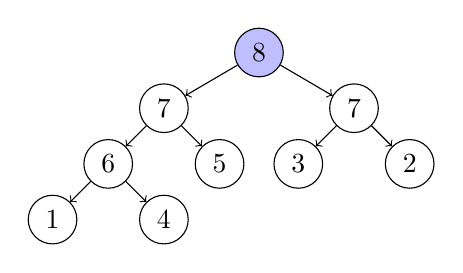
\begin{tikzpicture}[->,nodes={draw, circle}]
		\node (a8) [fill = blue!25] {8};
		\node (a6) [below left of = a8, xshift=-0.5cm] {7};
		\node (a7) [below right of = a8, xshift=0.5cm]{7};
		\node (a4) [below left of = a6]{6};
		\node (a5) [below right of = a6]{5};
		\node (a3) [below left of = a7]{3};
		\node (a2) [below right of = a7]{2};
		\node (a1) [below left of = a4]{1};
		\node (n7) [below right of = a4]{4};
		\draw (a8) -> (a7);
		\draw (a8) -> (a6); 
		\draw (a6) -> (a4);
		\draw (a6) -> (a5);
		\draw (a7) -> (a3);
		\draw (a7) -> (a2);
		\draw (a4) -> (a1);
		\draw (a4) -> (n7);
		\end{tikzpicture}
	\end{center}
\end{frame}

\begin{frame}
	\frametitle{Removing the first element}
	Step 2: put the last node at the root
	
	\begin{center}
		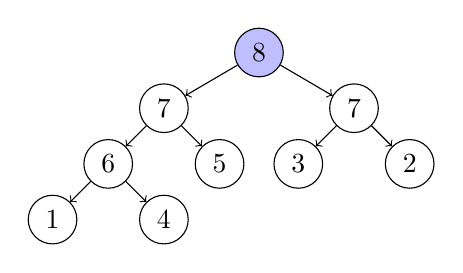
\begin{tikzpicture}[->,nodes={draw, circle}]
		\node (a8) [fill = blue!25] {8};
		\node (a6) [below left of = a8, xshift=-0.5cm] {7};
		\node (a7) [below right of = a8, xshift=0.5cm]{7};
		\node (a4) [below left of = a6]{6};
		\node (a5) [below right of = a6]{5};
		\node (a3) [below left of = a7]{3};
		\node (a2) [below right of = a7]{2};
		\node (a1) [below left of = a4]{1};
		\node (n7) [below right of = a4]{4};
		\draw (a8) -> (a7);
		\draw (a8) -> (a6); 
		\draw (a6) -> (a4);
		\draw (a6) -> (a5);
		\draw (a7) -> (a3);
		\draw (a7) -> (a2);
		\draw (a4) -> (a1);
		\draw (a4) -> (n7);
		\end{tikzpicture}
	\end{center}
\end{frame}

\begin{frame}
	\frametitle{Removing the first element}
	Step 2: put the last node at the root
	
	\begin{center}
		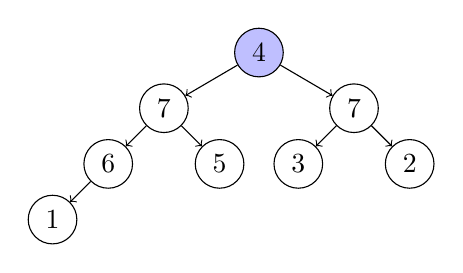
\begin{tikzpicture}[->,nodes={draw, circle}]
		\node (a8) [fill = blue!25] {4};
		\node (a6) [below left of = a8, xshift=-0.5cm] {7};
		\node (a7) [below right of = a8, xshift=0.5cm]{7};
		\node (a4) [below left of = a6]{6};
		\node (a5) [below right of = a6]{5};
		\node (a3) [below left of = a7]{3};
		\node (a2) [below right of = a7]{2};
		\node (a1) [below left of = a4]{1};
		\draw (a8) -> (a7);
		\draw (a8) -> (a6); 
		\draw (a6) -> (a4);
		\draw (a6) -> (a5);
		\draw (a7) -> (a3);
		\draw (a7) -> (a2);
		\draw (a4) -> (a1);
		\end{tikzpicture}
	\end{center}
\end{frame}

\begin{frame}
	\frametitle{Removing the first element}
	Step 3: check heap property with the children of the node.\\
	\only<2>{\textbf{Not respected -> swap with (the first) 7}}
	\begin{center}
		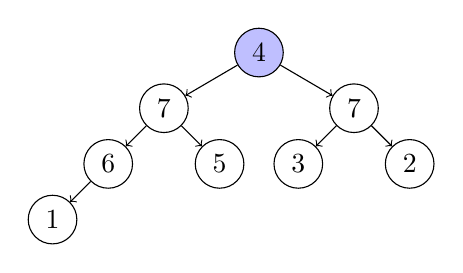
\begin{tikzpicture}[->,nodes={draw, circle}]
		\node (a8) [fill = blue!25] {4};
		\node (a6) [below left of = a8, xshift=-0.5cm] {7};
		\node (a7) [below right of = a8, xshift=0.5cm]{7};
		\node (a4) [below left of = a6]{6};
		\node (a5) [below right of = a6]{5};
		\node (a3) [below left of = a7]{3};
		\node (a2) [below right of = a7]{2};
		\node (a1) [below left of = a4]{1};
		\draw (a8) -> (a7);
		\draw (a8) -> (a6); 
		\draw (a6) -> (a4);
		\draw (a6) -> (a5);
		\draw (a7) -> (a3);
		\draw (a7) -> (a2);
		\draw (a4) -> (a1);
		\end{tikzpicture}
	\end{center}
\end{frame}

\begin{frame}
	\frametitle{Removing the first element}
	Step 3: check heap property with the children of the node.\\
	\textbf{Not respected -> swap with (the first) 7}
	\begin{center}
		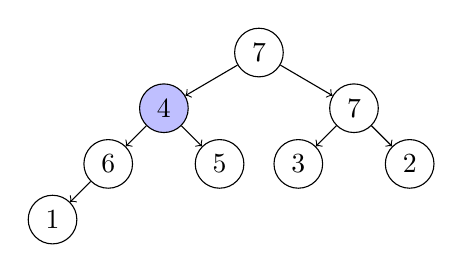
\begin{tikzpicture}[->,nodes={draw, circle}]
		\node (a8) [] {7};
		\node (a6) [below left of = a8, xshift=-0.5cm,fill = blue!25] {4};
		\node (a7) [below right of = a8, xshift=0.5cm]{7};
		\node (a4) [below left of = a6]{6};
		\node (a5) [below right of = a6]{5};
		\node (a3) [below left of = a7]{3};
		\node (a2) [below right of = a7]{2};
		\node (a1) [below left of = a4]{1};
		\draw (a8) -> (a7);
		\draw (a8) -> (a6); 
		\draw (a6) -> (a4);
		\draw (a6) -> (a5);
		\draw (a7) -> (a3);
		\draw (a7) -> (a2);
		\draw (a4) -> (a1);
		\end{tikzpicture}
	\end{center}
\end{frame}

\begin{frame}
	\frametitle{Removing the first element}
	Step 3: check heap property with the children of the node.\\
	\textbf{Not respected -> swap with 6 (the greatest child)}
	\begin{center}
		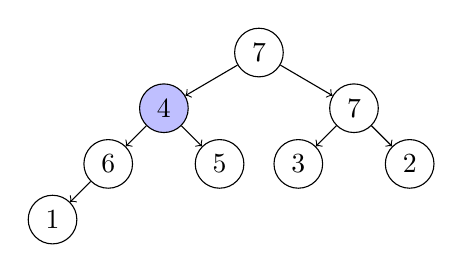
\begin{tikzpicture}[->,nodes={draw, circle}]
		\node (a8) [] {7};
		\node (a6) [below left of = a8, xshift=-0.5cm,fill = blue!25] {4};
		\node (a7) [below right of = a8, xshift=0.5cm]{7};
		\node (a4) [below left of = a6]{6};
		\node (a5) [below right of = a6]{5};
		\node (a3) [below left of = a7]{3};
		\node (a2) [below right of = a7]{2};
		\node (a1) [below left of = a4]{1};
		\draw (a8) -> (a7);
		\draw (a8) -> (a6); 
		\draw (a6) -> (a4);
		\draw (a6) -> (a5);
		\draw (a7) -> (a3);
		\draw (a7) -> (a2);
		\draw (a4) -> (a1);
		\end{tikzpicture}
	\end{center}
\end{frame}

\begin{frame}
	\frametitle{Removing the first element}
	Step 3: check heap property with the children of the node.\\
	\textbf{Not respected -> swap with 6 (the greatest child)}
	\begin{center}
		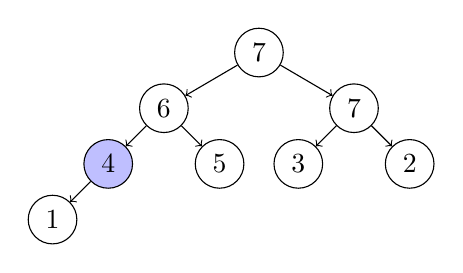
\begin{tikzpicture}[->,nodes={draw, circle}]
		\node (a8) [] {7};
		\node (a6) [below left of = a8, xshift=-0.5cm] {6};
		\node (a7) [below right of = a8, xshift=0.5cm]{7};
		\node (a4) [below left of = a6,fill = blue!25]{4};
		\node (a5) [below right of = a6]{5};
		\node (a3) [below left of = a7]{3};
		\node (a2) [below right of = a7]{2};
		\node (a1) [below left of = a4]{1};
		\draw (a8) -> (a7);
		\draw (a8) -> (a6); 
		\draw (a6) -> (a4);
		\draw (a6) -> (a5);
		\draw (a7) -> (a3);
		\draw (a7) -> (a2);
		\draw (a4) -> (a1);
		\end{tikzpicture}
	\end{center}
\end{frame}

\begin{frame}
	\frametitle{Removing the first element}
	Step 3: check heap property with the children of the node.\\
	\textbf{Done}
	\begin{center}
		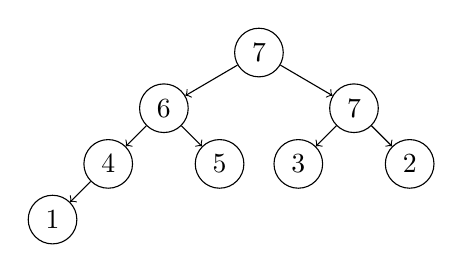
\begin{tikzpicture}[->,nodes={draw, circle}]
		\node (a8) [] {7};
		\node (a6) [below left of = a8, xshift=-0.5cm] {6};
		\node (a7) [below right of = a8, xshift=0.5cm]{7};
		\node (a4) [below left of = a6]{4};
		\node (a5) [below right of = a6]{5};
		\node (a3) [below left of = a7]{3};
		\node (a2) [below right of = a7]{2};
		\node (a1) [below left of = a4]{1};
		\draw (a8) -> (a7);
		\draw (a8) -> (a6); 
		\draw (a6) -> (a4);
		\draw (a6) -> (a5);
		\draw (a7) -> (a3);
		\draw (a7) -> (a2);
		\draw (a4) -> (a1);
		\end{tikzpicture}
	\end{center}
\end{frame}

\begin{frame}
	\frametitle{Usage}
	\begin{itemize}
		\item Priority queues
		\item Dijkstra
		\item Sorting
		\item ...
	\end{itemize}
	
	\begin{itemize}
		\item In C++: std::priority\_queue
		\item In Java: PriorityQueue
	\end{itemize}
\end{frame}